\documentclass[10pt,a4paper]{article}

\usepackage[utf8]{inputenc}
\usepackage[T1]{fontenc}
\usepackage[brazil]{babel}
\usepackage{amsmath,amssymb}
\usepackage{graphicx}
\usepackage[colorlinks=true,linkcolor=blue,citecolor=blue,urlcolor=blue]{hyperref}
\usepackage{float}
\usepackage{subcaption}
\usepackage{booktabs}
\usepackage{geometry}
\usepackage{xcolor}
\usepackage{titlesec}

\geometry{top=1.8cm, bottom=1.8cm, left=2cm, right=2cm}
\setlength{\parskip}{2pt}
\setlength{\parindent}{0pt}
\setlength{\abovecaptionskip}{4pt}
\setlength{\belowcaptionskip}{2pt}
\titlespacing{\section}{0pt}{8pt}{4pt}
\titlespacing{\subsection}{0pt}{6pt}{2pt}

\renewcommand{\figurename}{Figura}
\renewcommand{\tablename}{Tabela}

\title{Projeto 04: Desafio Kaggle de Classificação\\ \large Home Credit Default Risk --- Predição de Inadimplência de Crédito}
\author{
  \small
  Rodrigo Banin Ferraz de Camargo (238257)
  \textbullet{}
    Caio Lima Albulquerque (288808) \\ \small Ricardo Andrade Oliveira Bello (247326)
  \date{\small\today}
}
\begin{document}

\maketitle

\section{Descrição do Problema}
Este projeto aborda a competição \textit{Home Credit Default Risk}\footnote{\url{https://www.kaggle.com/competitions/home-credit-default-risk}} do Kaggle, cujo objetivo é prever a probabilidade de um cliente se tornar inadimplente (\textit{default}) em um empréstimo. O desafio trata-se de um problema de \textbf{classificação binária} amparado por um conjunto de dados substancial (\textbf{307.511} exemplos de treino e \textbf{48.744} de teste) e avaliado pela \textbf{métrica oficial ROC AUC}. Essa métrica é ideal para o contexto da competição, que é caracterizado por um \textbf{desbalanceamento severo} de classes, com apenas $\sim$8,1\% de inadimplentes (variável \texttt{TARGET} igual a 1).

A base de dados é realista e estruturada em \textbf{sete tabelas relacionais}, o que impõe o desafio técnico de consolidar informações financeiras dispersas --- como histórico no bureau de crédito, pedidos anteriores e pagamentos de parcelas --- em um único vetor de atributos por cliente. Para solucionar o problema comparando mais de três metodologias, a estratégia utilizada combinou engenharia de atributos agressiva sobre as tabelas suplementares, avaliação de seis modelos-base distintos (incluindo regressão logística, floresta aleatória, redes neurais e \textit{gradient boosting}), e a consolidação das previsões em um \textit{ensemble} ponderado. O trabalho também contempla análises profundas de interpretabilidade (utilizando SHAP) e limitações da abordagem, culminando na submissão final registrada no arquivo \texttt{submission.csv}.

\section{Análise Exploratória de Dados}
A análise estrutural do conjunto de dados revelou um desbalanceamento acentuado na variável alvo (Figura~\ref{fig:eda-dist}a), em que apenas $\sim$8,1\% dos clientes são inadimplentes (uma proporção de 1 para 12). Esse cenário torna a acurácia uma métrica enganosa --- visto que um classificador trivial que preveja invariavelmente a classe majoritária alcançaria $\sim$91,9\% de acurácia --- justificando a adoção da métrica ROC AUC e de técnicas de rebalanceamento de classes na modelagem.

A investigação das variáveis preditivas evidenciou forte sinal discriminatório em atributos numéricos e categóricos. Fontes externas de crédito (como \texttt{EXT\_SOURCE\_2}) exibem distribuições nitidamente deslocadas para valores menores entre os inadimplentes, concentrando o maior risco (Figura~\ref{fig:eda-dist}b). 

\begin{figure}[H]
    \centering
    \begin{subfigure}[b]{0.48\textwidth}
        \centering
        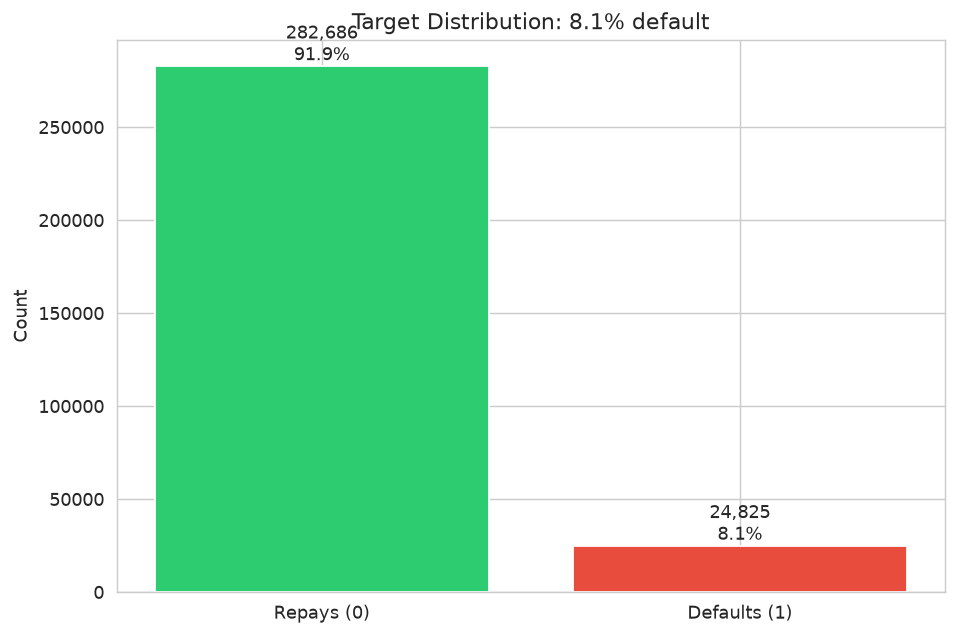
\includegraphics[width=\textwidth]{images/eda_target_distribution.png}
        \caption{Distribuição da variável alvo (\texttt{TARGET}).}
        \label{fig:eda-target}
    \end{subfigure}
    \hfill
    \begin{subfigure}[b]{0.48\textwidth}
        \centering
        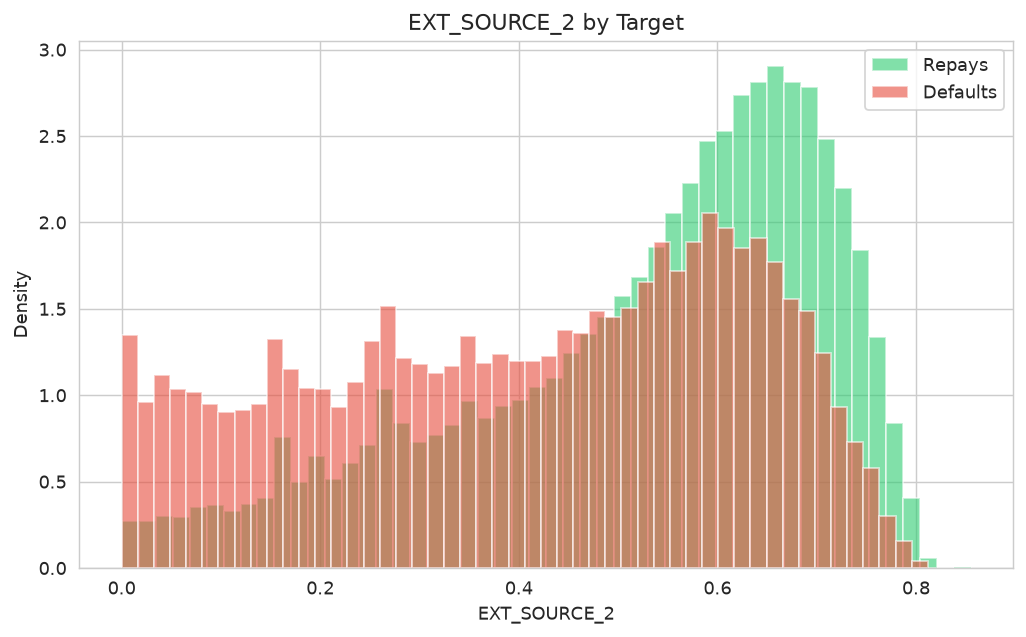
\includegraphics[width=\textwidth]{images/eda_ext_source_2_by_target.png}
        \caption{Comportamento de \texttt{EXT\_SOURCE\_2} por classe.}
        \label{fig:ext-source}
    \end{subfigure}
    \caption{Análise de desbalanceamento do alvo e comportamento discriminatório do \textit{score} externo de crédito.}
    \label{fig:eda-dist}
\end{figure}
\newpage
Paralelamente, observou-se uma relação inversa entre a idade do cliente e o risco de crédito, com a taxa de \textit{default} superando a média populacional entre indivíduos mais jovens (Figura~\ref{fig:eda-features}a). Variáveis categóricas, como o nível de escolaridade (Figura~\ref{fig:eda-features}b), gênero e tipo de renda, também demonstraram desvios significativos em relação à taxa base de 8,1\%, confirmando seu valor preditivo. Por outro lado, o valor bruto do crédito solicitado apresentou forte sobreposição entre as classes, revelando-se um preditor fraco de forma isolada, o que demandou a criação de razões financeiras na etapa de engenharia de atributos.

\begin{figure}[H]
    \centering
    \begin{subfigure}[b]{0.48\textwidth}
        \centering
        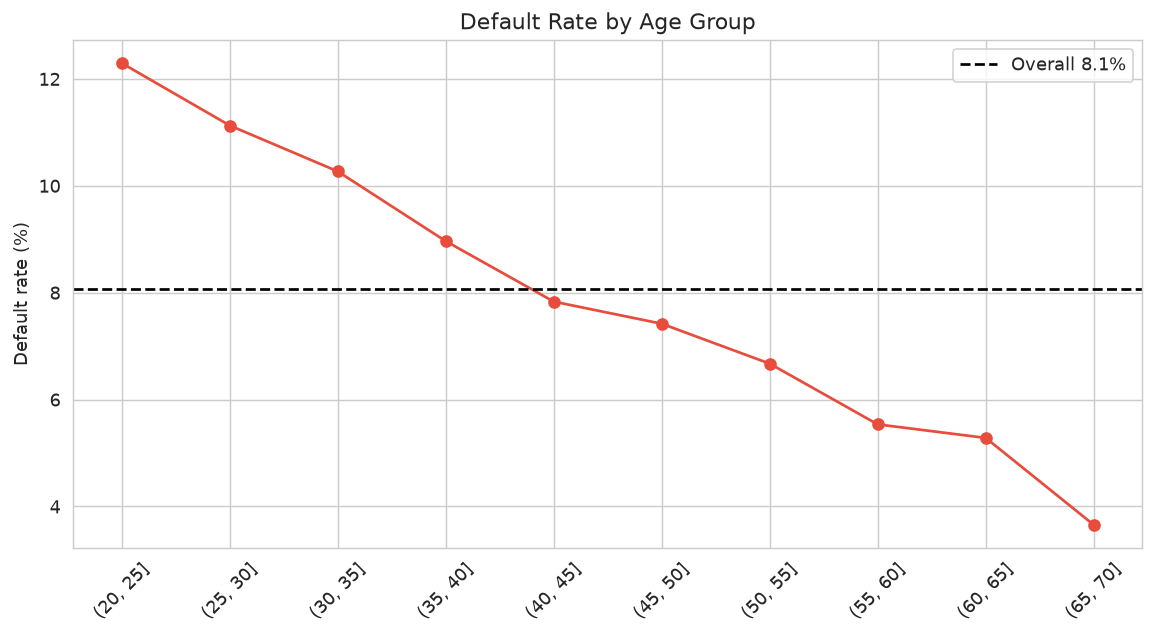
\includegraphics[width=\textwidth]{images/eda_default_rate_by_age.png}
        \caption{Taxa de \textit{default} por faixa etária.}
        \label{fig:age-rate}
    \end{subfigure}
    \hfill
    \begin{subfigure}[b]{0.48\textwidth}
        \centering
        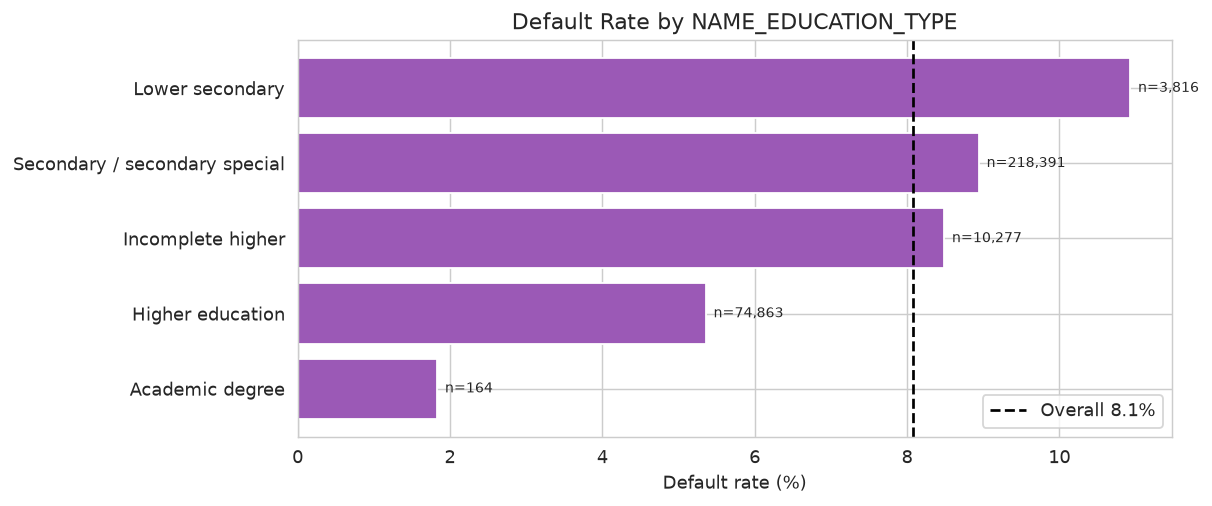
\includegraphics[width=\textwidth]{images/eda_default_rate_name_education_type.png}
        \caption{Taxa de \textit{default} por nível de escolaridade.}
        \label{fig:education-rate}
    \end{subfigure}
    \caption{Comportamento da taxa de inadimplência de acordo com atributos demográficos e socioeconômicos.}
    \label{fig:eda-features}
\end{figure}

\section{Engenharia de Atributos e Pré-processamento}
Visto que os algoritmos de estado da arte para dados tabulares pertencem majoritariamente à mesma família de \textit{gradient boosting}, o diferencial de desempenho neste desafio reside na \textbf{engenharia de atributos}, e não na escolha do modelo isoladamente. O obstáculo técnico consiste em condensar históricos relacionais de tamanho variável (múltiplos empréstimos anteriores, registros de bureau e parcelas mensais) em um vetor de características de dimensão fixa por cliente (\texttt{SK\_ID\_CURR}). 

Para isso, foram estruturadas agregações estatísticas (\texttt{groupby} aplicando média, mínimo, máximo, soma e contagem) sobre as cinco tabelas suplementares, destacando-se as seguintes frentes:
\begin{itemize}
    \item \textbf{Bureau (\texttt{BUR\_*})} e \textbf{Balanço (\texttt{bureau\_balance})}: Sumarização de saldos devedores, dias em atraso e volume de créditos ativos. As \textit{flags} de status mensal foram agregadas por \textit{one-hot} seguido de média, capturando a fração de meses em inadimplência.
    \item \textbf{Pedidos Anteriores (\texttt{PRV\_*})}: Métricas de valores propostos versus aprovados e, crucialmente, as taxas de deferimento e rejeição (\texttt{PRV\_APPROVED\_RATIO}, \texttt{PRV\_REFUSED\_RATIO}), mapeando o histórico de crédito na própria instituição.
    \item \textbf{Histórico de Parcelas (\texttt{INS\_*})}: Indicadores de pontualidade e comportamento financeiro, incluindo a razão de pagamento (\texttt{INS\_PAYMENT\_RATIO}), atraso médio em dias (\texttt{INS\_LATE\_DAYS\_MEAN}) e a discrepância média de valores (\texttt{INS\_PAYMENT\_DIFF\_MEAN}).
    \item \textbf{Tabela Principal}: Injeção de conhecimento de domínio através de interações e razões financeiras cruciais, como o cruzamento do escore externo com a idade (\texttt{EXT\_SOURCE\_MEAN\_x\_AGE}), índices de endividamento, razão crédito/renda e a taxa de ciclo de vida (tempo de emprego relativo à idade).
\end{itemize}

O processo de fusão expandiu o espaço de características de $\sim$120 para \textbf{$\sim$350 atributos}, acionando um pipeline de pré-processamento padronizado: (i) \textit{Label Encoding} homogêneo das variáveis categóricas via ajuste conjunto sobre treino e teste; (ii) \textbf{imputação pela mediana} para tratar dados faltantes de forma robusta a \textit{outliers} e assimetrias; (iii) conversão tipográfica para \texttt{float32}, reduzindo em 50\% o consumo de RAM; (iv) remoção de colunas redundantes ou quase-constantes via \textbf{filtro de variância} (\texttt{VarianceThreshold} $= 0{,}001$); e (v) \textbf{escalonamento robusto} (\texttt{RobustScaler}, baseado em mediana e IQR) aplicado estritamente aos modelos sensíveis à escala (regressão logística e rede neural), preservando a invariância monotônica original para os modelos de árvore. 

Embora robusta, essa abordagem consolidada por cliente adota uma postura conservadora se comparada às soluções do topo do Kaggle, que exploram janelas temporais móveis, recência de atrasos e razões cruzadas inter-tabelas --- oportunidades de melhoria detalhadas na Seção~8.

\section{Modelagem e Estratégia de Validação}
Foram avaliados \textbf{seis modelos-base} distintos sob um protocolo de \textbf{validação cruzada estratificada em 5 folds}, garantindo a preservação da proporção original de classes em todas as partições. O desempenho de cada classificador foi mensurado via previsões \textit{out-of-fold} (OOF) para mitigar qualquer risco de vazamento de dados (\textit{data leakage}), enquanto as predições finais de teste consistiram na média das probabilidades geradas por cada fold.

O desbalanceamento foi tratado de maneira nativa em cada ecossistema: aplicou-se peso positivo proporcional ($\approx 11{,}4$) nos \textit{boosters}, pesos balanceados por subamostragem na floresta aleatória, e amostragem ponderada combinada a \texttt{pos\_weight} na rede neural. Os paradigmas testados compreenderam:
\begin{itemize}
    \item \textbf{Regressão Logística (Linha de Base):} Modelo linear simples ajustado sobre dados escalonados para estabelecer o piso de desempenho preditivo do experimento.
    \item \textbf{XGBoost / LightGBM / CatBoost:} Três implementações distintas de \textit{gradient boosting} com filosofias complementares (crescimento por nível, crescimento por folha e tratamento nativo de variáveis categóricas, respectivamente). Foram parametrizados com até 4.000 iterações, \texttt{learning\_rate} $=0{,}03$, regularização e critério de parada precoce (\textit{early stopping}) entre 150 e 200 rodadas.
    \item \textbf{Random Forest:} Abordagem de \textit{bagging} estruturada com 150 árvores independentes (profundidade 12 e mínimo de 30 amostras por folha). Por construir estimadores isolados via amostras \textit{bootstrap}, gerou erros descorrelacionados em relação aos \textit{boosters}, injetando diversidade ao experimento.
    \item \textbf{Rede Neural Profunda (PyTorch):} Um Perceptron Multicamadas (MLP) \textit{feedforward} configurado com topologia $[512, 256, 128, 64]$, camadas de \textit{BatchNorm}, \textit{Dropout} de 0,3 para regularização, otimizador \texttt{AdamW} e agendador dinâmico \texttt{ReduceLROnPlateau}.
\end{itemize}

Visando contrair a variância global e extrair o potencial preditivo máximo, consolidou-se os modelos não lineares por meio de uma média ponderada de suas probabilidades OOF (a regressão logística foi descartada devido ao seu fraco desempenho). A distribuição de pesos priorizou os algoritmos preditivamente dominantes, mas preservou a contribuição de famílias estatísticas distintas para garantir resiliência e estabilidade ao conjunto: LightGBM (0,30), XGBoost (0,28), CatBoost (0,27), Random Forest (0,10) e Rede Neural (0,05).

\section{Resultados e Comparação de Modelos}
Os resultados consolidados via validação cruzada \textit{out-of-fold} (OOF) e o respectivo desempenho preditivo estão sumarizados na Tabela~\ref{tab:comparison}. Na execução final, o \textbf{XGBoost} alcançou a maior robustez métrica individual, registrando uma AUC OOF de \textbf{0,7876}. O \textbf{Ensemble} ponderado obteve um desempenho de ordenação virtualmente empatado (\textbf{0,7865}), mas superou todos os classificadores isolados na métrica de \textbf{\textit{Average Precision} (AP)}, atingindo \textbf{0,2832} --- um ganho expressivo dada a natureza desbalanceada do problema.

Esse patamar de desempenho convergiu de forma consistente no ambiente de testes do Kaggle, resultando em um escore privado de \textbf{0,78173} e público de \textbf{0,7828} via arquivo \texttt{submission.csv}. Frente às soluções líderes da competição, historicamente estabelecidas em torno de \textbf{0,805} de AUC, a arquitetura desenvolvida posicionou-se no \textbf{top 38\%} do ranking geral ($\sim$3.000ª colocação entre 8.000 participantes). A distância de aproximadamente 0,02 ponto de AUC em relação ao topo confirma a hipótese central deste experimento: os modelos baseados em árvores já operam no limite estatístico do estado da arte tabular, e o incremento residual remanescente depende da profundidade empírica da engenharia de atributos relacionais, não da alternância de algoritmos.

\begin{table}[H]
    \centering
    \small
    \begin{tabular}{lcc}
        \toprule
        Modelo & AUC OOF & AP OOF \\
        \midrule
        XGBoost                  & \textbf{0,7876} & 0,2813 \\
        LightGBM                 & 0,7867          & 0,2803 \\
        Ensemble                 & 0,7865          & \textbf{0,2832} \\
        CatBoost                 & 0,7861          & 0,2807 \\
        Random Forest            & 0,7599          & 0,2437 \\
        Deep Learning (NN)       & 0,6252          & 0,1335 \\
        Regressão Logística      & 0,4902          & 0,0776 \\
        \bottomrule
    \end{tabular}
    \caption{AUC e \textit{Average Precision} \textit{out-of-fold} obtidas com validação cruzada em 5 folds.}
    \label{tab:comparison}
\end{table}

A hierarquia competitiva revelada na Figura~\ref{fig:model-perf} evidencia o domínio dos métodos de \textit{gradient boosting} (XGBoost, LightGBM e CatBoost), que formaram um bloco de vanguarda estatisticamente parelho ($\sim$0,786 - 0,788). A \textit{Random Forest} posicionou-se logo atrás (0,7599), apresentando uma retração esperada para algoritmos de \textit{bagging} frente ao \textit{boosting}, mas consolidando-se como um elemento crucial de diversidade para o metamodelo. 

Em contrapartida, a Rede Neural MLP exibiu um comportamento decepcionante (0,6252), reiterando a dificuldade de topologias \textit{feedforward} densas em mapear dados tabulares esparsos e de escalas mistas sem camadas de incorporação (\textit{embeddings}) especializadas. Por fim, a Regressão Logística performou abaixo do acaso (0,4902), atestando de forma empírica que a relação entre o perfil histórico relacional do cliente e o risco de inadimplência é governada por interações estritamente não lineares.

\begin{figure}[H]
    \centering
    \begin{subfigure}[b]{0.48\textwidth}
        \centering
        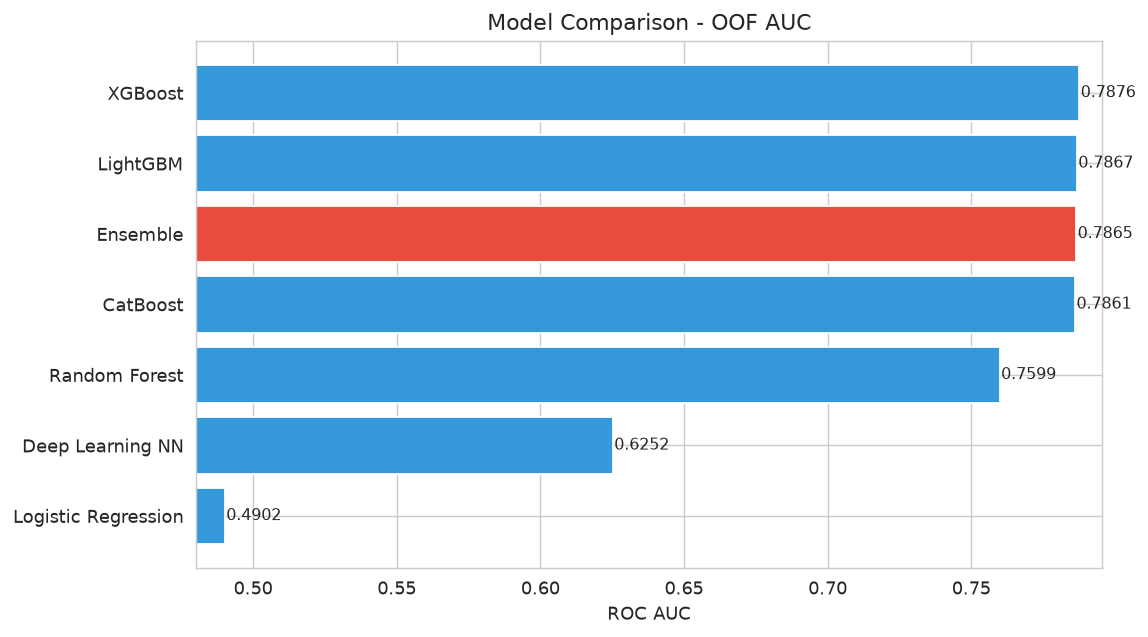
\includegraphics[width=\textwidth]{images/model_comparison.png}
        \caption{Comparação visual de AUC OOF.}
        \label{fig:model-comp}
    \end{subfigure}
    \hfill
    \begin{subfigure}[b]{0.48\textwidth}
        \centering
        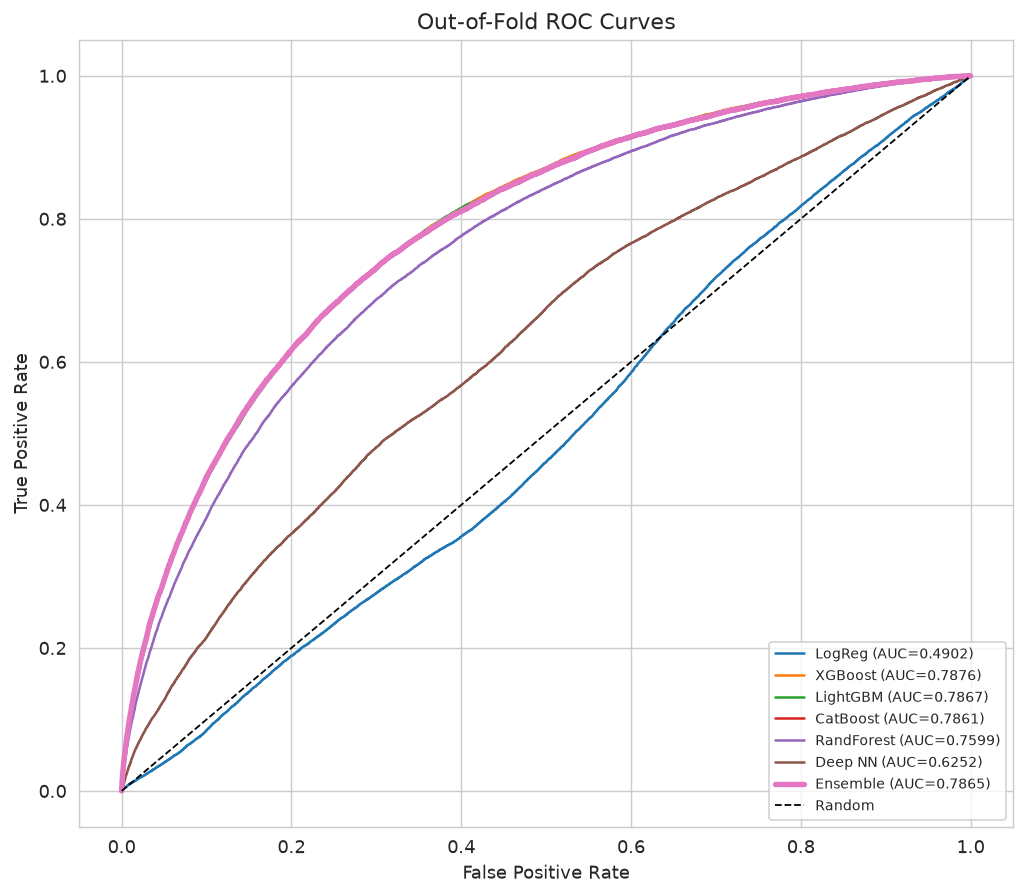
\includegraphics[width=\textwidth]{images/roc_curves.png}
        \caption{Curvas ROC OOF por modelo.}
        \label{fig:roc}
    \end{subfigure}
    \caption{Métricas globais de ordenação e curvas de sensibilidade discriminatória entre os modelos testados.}
    \label{fig:model-perf}
\end{figure}

A análise de separação de classes (Figura~\ref{fig:ensemble-diag}b) exibe um claro deslocamento direcional da classe de risco para a direita; contudo, a persistência de uma zona de sobreposição central reflete o limite intrínseco de separabilidade fixado no teto atual de AUC. Sob a ótica de correlação linear de predições (Figura~\ref{fig:ensemble-diag}c), comprova-se o forte acoplamento entre os três \textit{boosters} ($\sim$0,98), enquanto a \textit{Random Forest} apresenta menor colinearidade ($\sim$0,88), justificando sua inclusão no amortecimento da variância do \textit{blend}. Por fim, ressalta-se que as probabilidades brutas geradas não se encontram calibradas em termos absolutos em decorrência do rebalanceamento artificial via pesos de classe (\texttt{pos\_weight}). Como a métrica oficial (AUC) depende exclusivamente da ordenação ordinal relativa, essa distorção escalar não penaliza a performance competitiva, embora uma etapa subsequente de calibração (isotônica ou Platt) fosse mandatória para subsidiar estratégias reais de tomada de decisão de crédito.

\begin{figure}[H]
    \centering
    \begin{subfigure}[b]{0.35\textwidth}
        \centering
        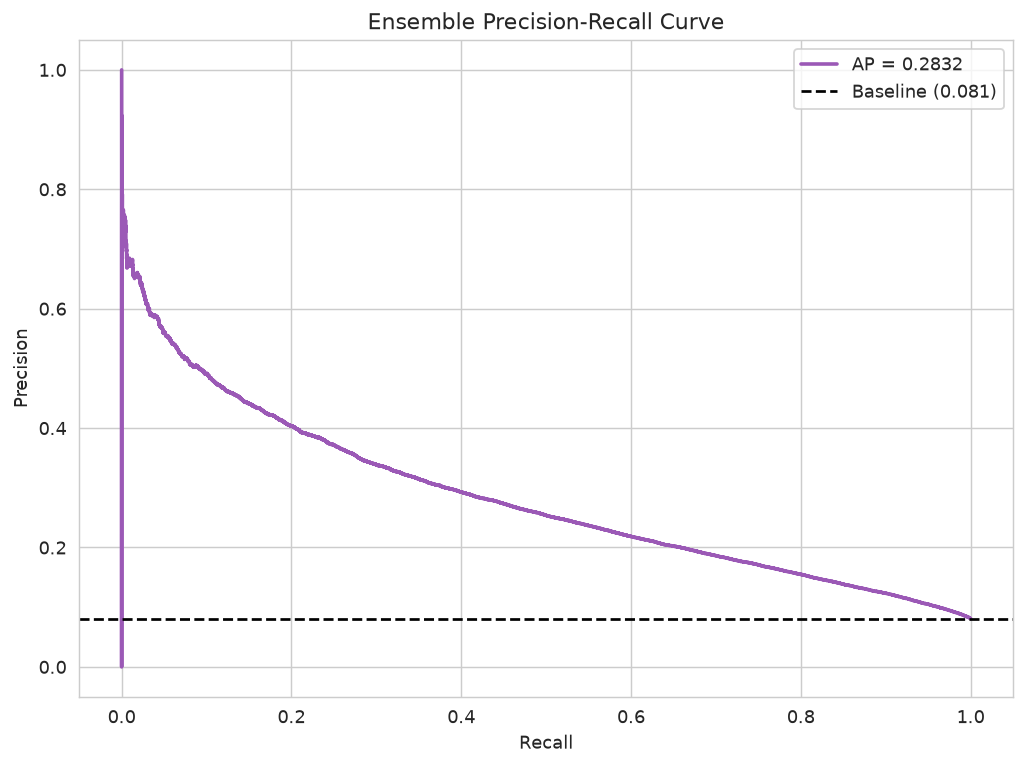
\includegraphics[width=\textwidth]{images/ensemble_precision_recall_curve.png}
        \caption{Curva Precisão-Recall do ensemble.}
        \label{fig:pr-ensemble}
    \end{subfigure}
    \hfill
    \begin{subfigure}[b]{0.35\textwidth}
        \centering
        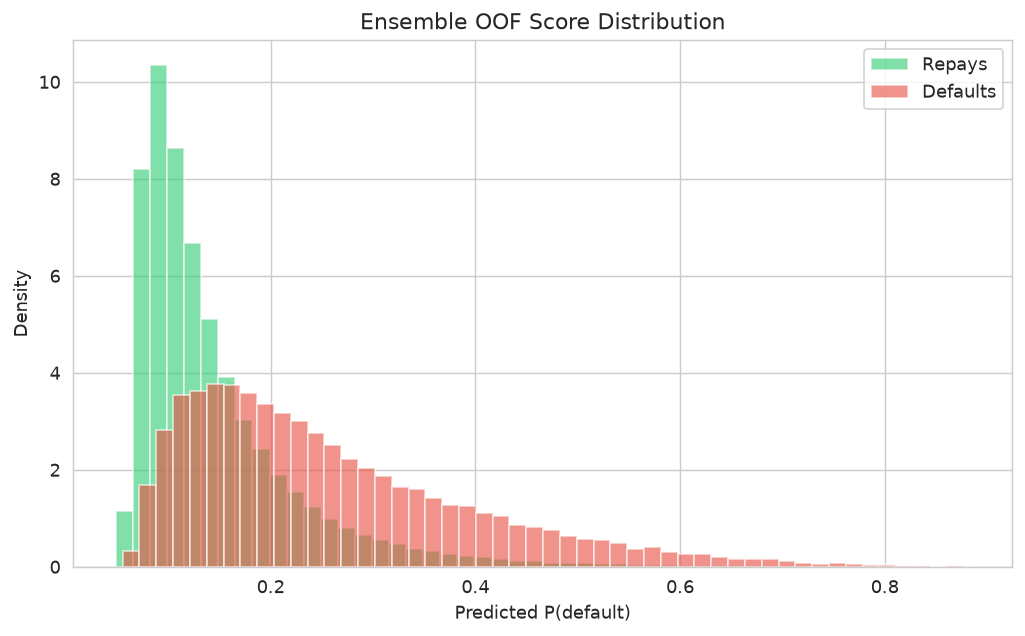
\includegraphics[width=\textwidth]{images/ensemble_score_distribution.png}
        \caption{Distribuição de escores por classe real.}
        \label{fig:score-dist}
    \end{subfigure}
    \\ \vspace{6pt}
    \begin{subfigure}[b]{0.35\textwidth}
        \centering
        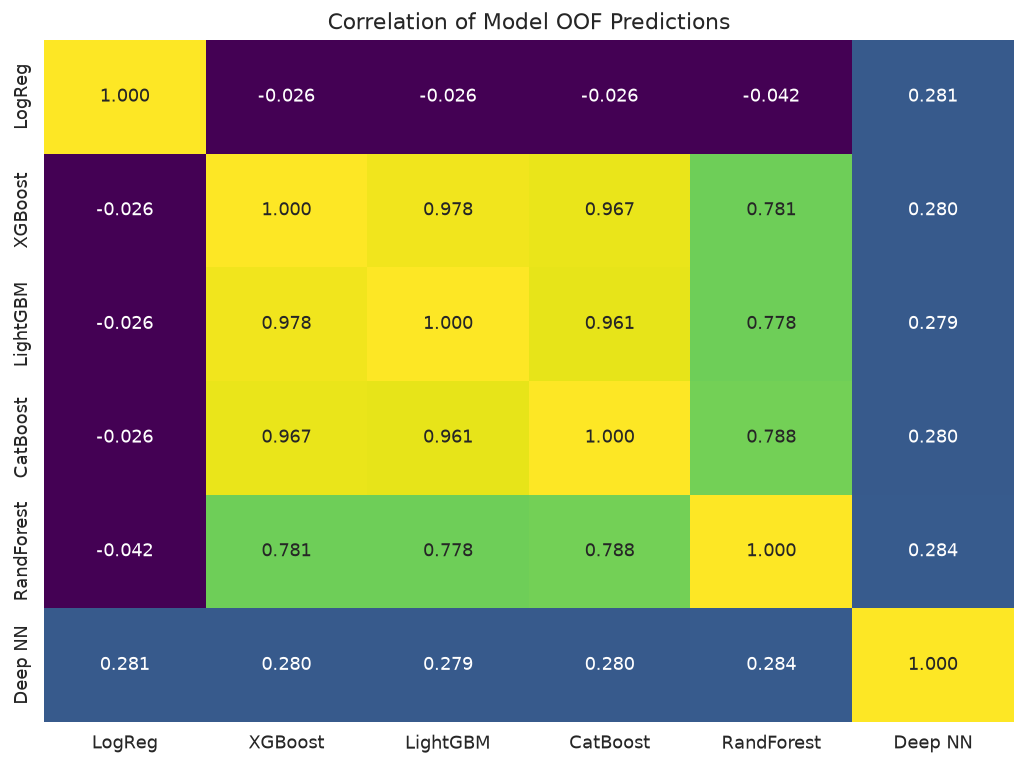
\includegraphics[width=\textwidth]{images/model_oof_correlation.png}
        \caption{Correlação entre as previsões OOF.}
        \label{fig:corr}
    \end{subfigure}
    \caption{Diagnósticos comportamentais, distribuição probabilística de risco e análise de diversidade interna do ensemble.}
    \label{fig:ensemble-diag}
\end{figure}

\section{Análise de Erros e Utilidade de Negócio}
Além da métrica estatística pura (AUC), a validação da solução sob a ótica de \textbf{utilidade de negócio} e aplicabilidade prática é fundamental, visto que escores de crédito operam prioritariamente na otimização e priorização de análises de risco. A ordenação dos clientes por \textbf{decis de risco} previstos revelou um comportamento monotônico exemplar (Figura~\ref{fig:business-metrics}c): a taxa real de inadimplência evolui de apenas \textbf{1,0\%} no decil de menor risco para expressivos \textbf{30,3\%} no decil mais crítico. Isso representa uma capacidade de concentração de risco no topo de aproximadamente \textbf{3,8$\times$} em relação à taxa base da população ($\sim$8,1\%), validando o valor operacional do modelo para subsidiar estratégias de triagem automatizada e revisão manual seletiva.

Essa eficiência macroeconômica é corroborada pelas curvas de ganho acumulado (Figura~\ref{fig:business-metrics}a) e de separação de Kolmogorov-Smirnov (KS) (Figura~\ref{fig:business-metrics}b). O \textit{ensemble} registrou um \textbf{índice KS de 0,432}, com o ponto de máxima separação estatística localizado precisamente em torno dos 31\% clientes classificados como mais propensos ao \textit{default}. Na prática bancária, direcionar os esforços de auditoria ou restringir a concessão de crédito a essa fatia específica captura uma parcela desproporcionalmente alta dos potenciais inadimplentes, minimizando perdas financeiras por real investido.

Por outro lado, a análise de limiares de decisão fixos (Figura~\ref{fig:business-metrics}d) ilustra o severo compromisso prático imposto pelo desbalanceamento da classe minoritária. O valor máximo de F1-Score obtido foi modesto, fixando-se em \textbf{0,340} sob um limiar de corte de \textbf{0,24}, associando uma precisão de 0,272 a um \textit{recall} de 0,453. Esse comportamento reitera que, neste domínio de problema, faz mais sentido estratégico utilizar o escore probabilístico contínuo como uma ferramenta de ordenação e ranqueamento de risco do que forçar uma decisão binária com limiar rígido. Embora a curva de Precisão-Recall aponte uma \textit{Average Precision} de 0,2832 --- substancialmente superior à linha de base aleatória de 0,081 --- a distância para o cenário ideal reflete a complexidade intrínseca da tarefa de crédito.

\begin{figure}[H]
    \centering
    \begin{subfigure}[b]{0.48\textwidth}
        \centering
        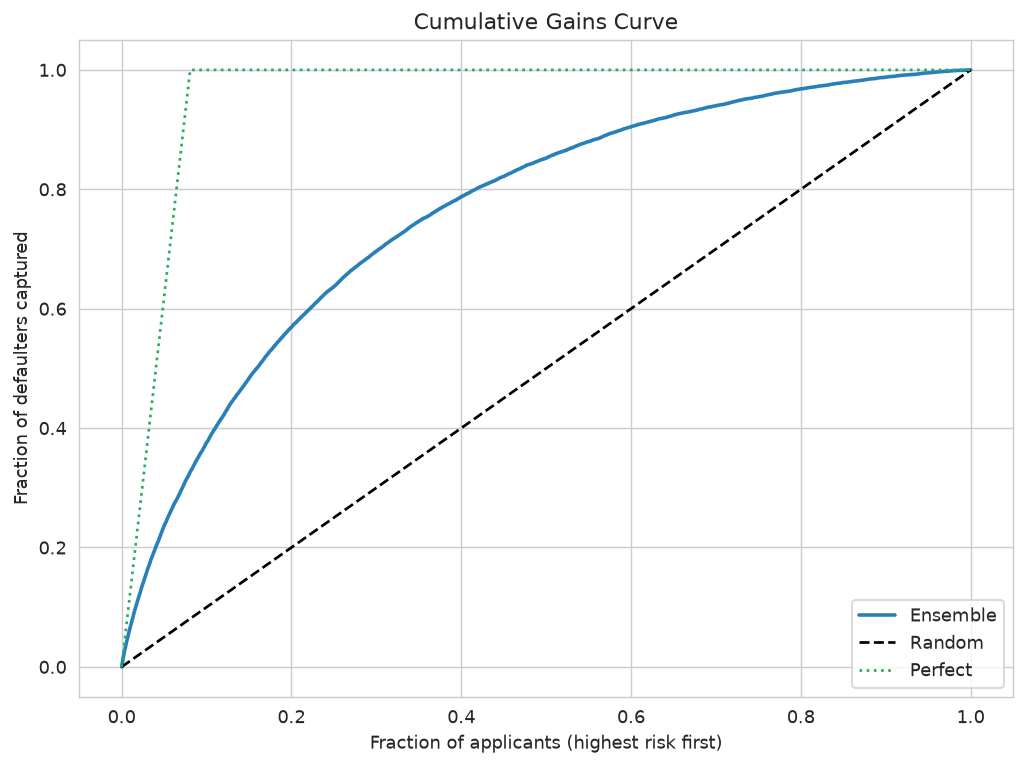
\includegraphics[width=\textwidth]{images/cumulative_gains_curve.png}
        \caption{Curva de ganho acumulado.}
        \label{fig:gains}
    \end{subfigure}
    \hfill
    \begin{subfigure}[b]{0.48\textwidth}
        \centering
        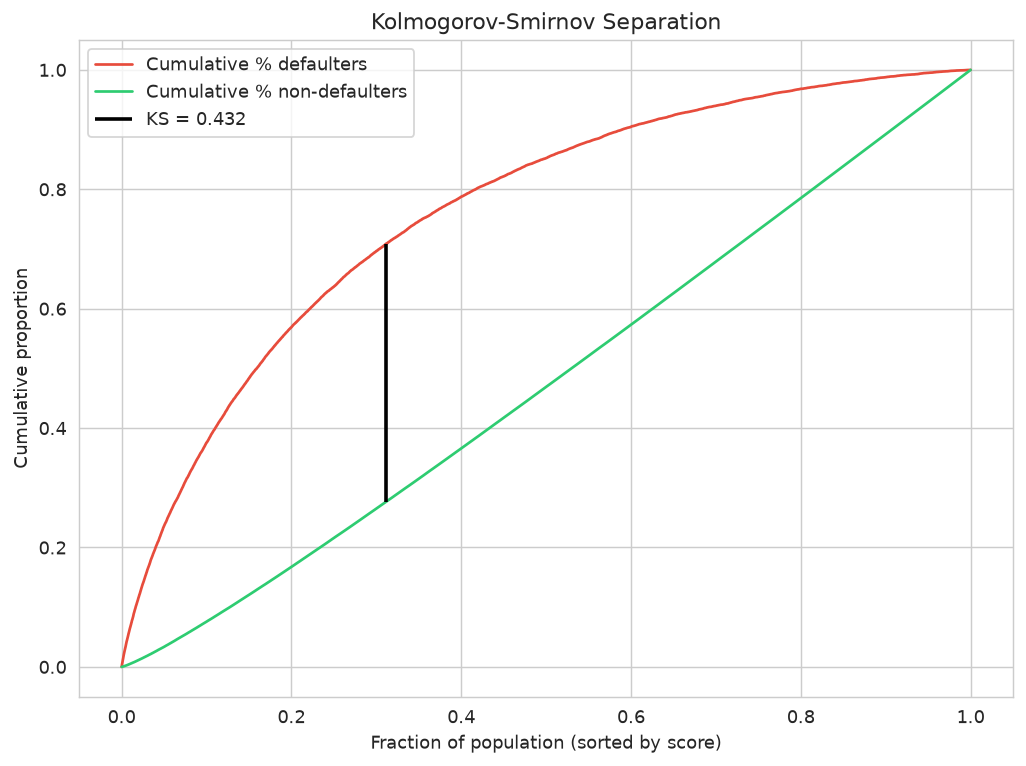
\includegraphics[width=\textwidth]{images/ks_curve.png}
        \caption{Curva de separação KS do ensemble.}
        \label{fig:ks}
    \end{subfigure}
    \\ \vspace{6pt}
    \begin{subfigure}[b]{0.48\textwidth}
        \centering
        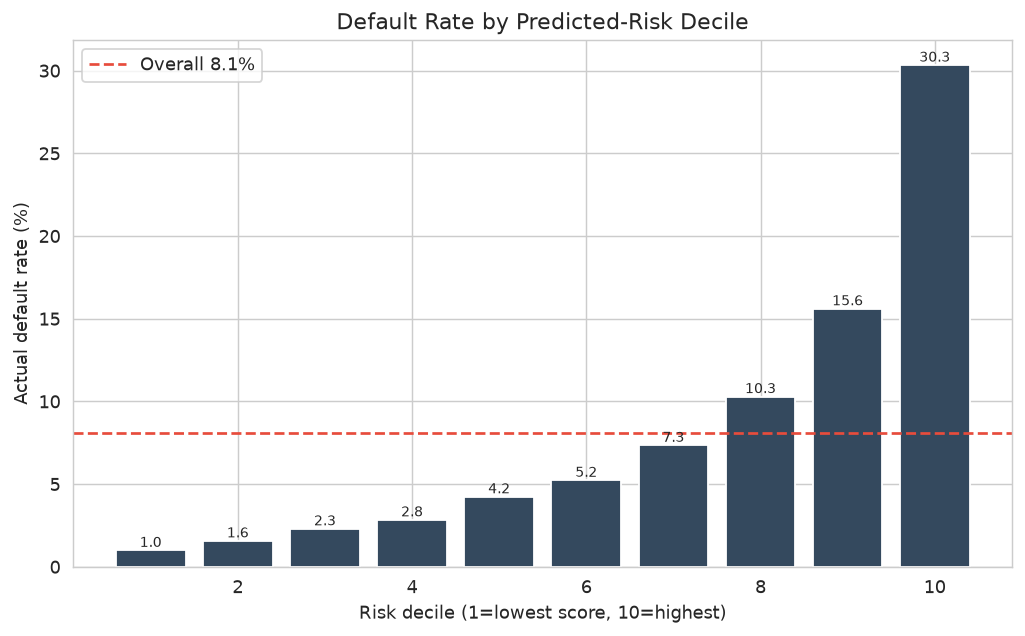
\includegraphics[width=\textwidth]{images/default_rate_by_risk_decile.png}
        \caption{Taxa de default por decil de risco.}
        \label{fig:decile}
    \end{subfigure}
    \hfill
    \begin{subfigure}[b]{0.48\textwidth}
        \centering
        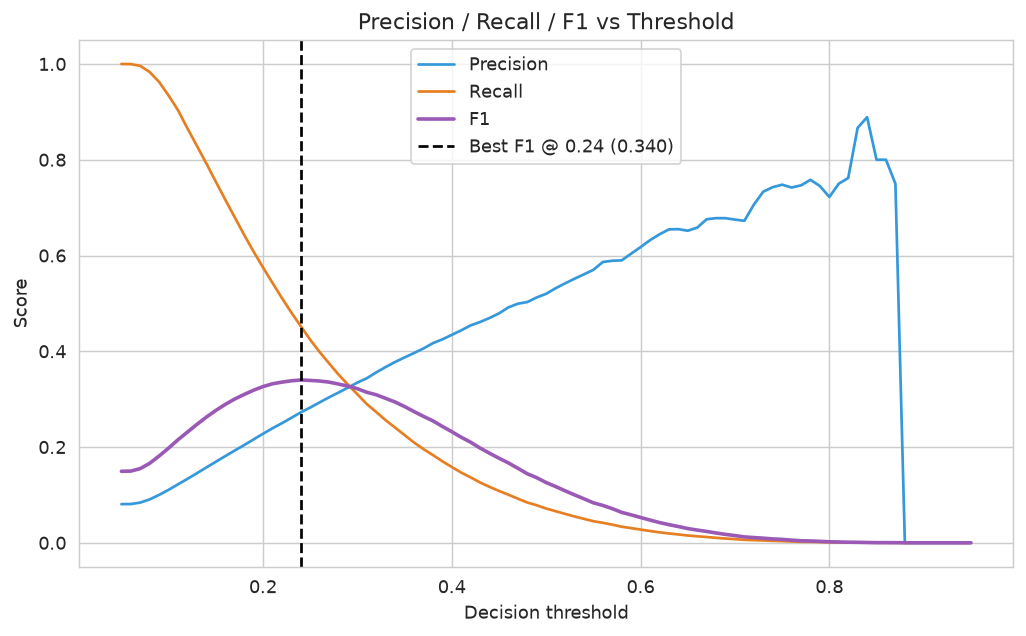
\includegraphics[width=\textwidth]{images/threshold_precision_recall_f1.png}
        \caption{Métricas por limiar de decisão.}
        \label{fig:threshold}
    \end{subfigure}
    \caption{Métricas de impacto de negócio, eficiência de ranqueamento por decis e análise de sensibilidade de limiares para o ensemble.}
    \label{fig:business-metrics}
\end{figure}
\newpage
\section{Interpretabilidade}
Para elucidar o processo de decisão do modelo e mitigar o risco de correlações espúrias comuns em dados tabulares relacionais, adotamos uma abordagem de interpretabilidade multidimensional. O pilar central foi o método SHAP (\textit{SHapley Additive exPlanations}), que decompõe a probabilidade prevista em contribuições marginais por atributo. Para garantir robustez empírica, cruzamos os valores SHAP com a importância por permutação, importância nativa dos modelos de árvore e a análise operacional de decis de risco, buscando consistência entre os diferentes métodos explicativos.

\begin{figure}[H]
    \centering
    \begin{subfigure}[b]{0.48\textwidth}
        \centering
        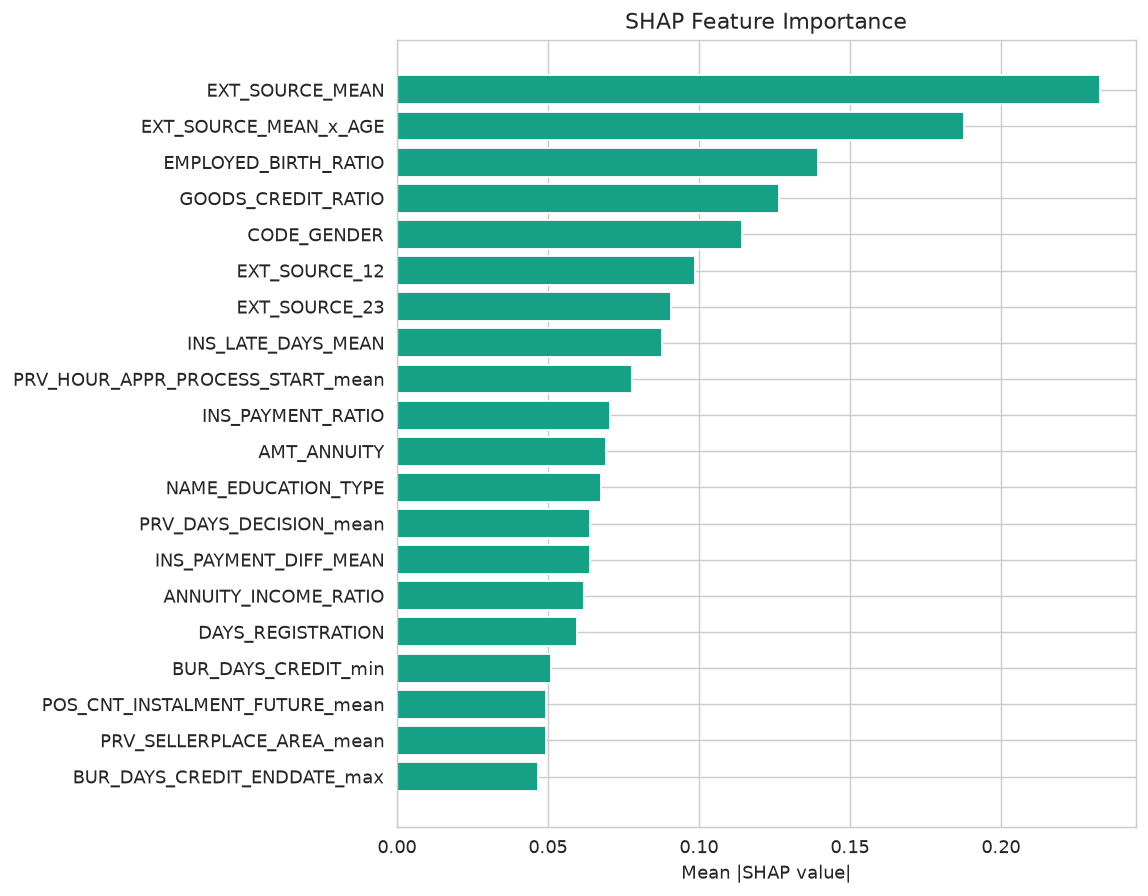
\includegraphics[width=\textwidth]{images/shap_feature_importance_single.png}
        \caption{Importância SHAP média dos atributos.}
        \label{fig:shap-importance}
    \end{subfigure}
    \hfill
    \begin{subfigure}[b]{0.48\textwidth}
        \centering
        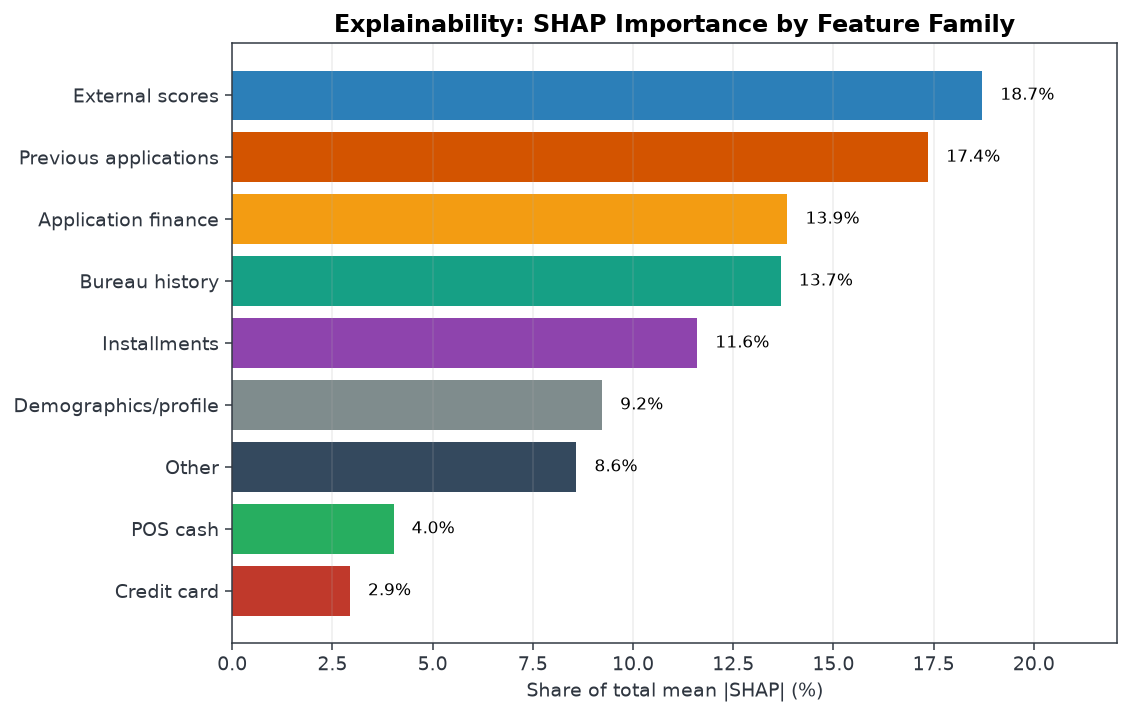
\includegraphics[width=\textwidth]{images/explainability_shap_group_importance.png}
        \caption{Importância agregada por família de origem.}
        \label{fig:shap-group-importance}
    \end{subfigure}
    \caption{Decomposição SHAP global indicando a predominância de fontes externas e atributos derivados.}
    \label{fig:shap-analysis}
\end{figure}

A análise SHAP (Figura~\ref{fig:shap-analysis}a) revela que as previsões são ancoradas prioritariamente nas fontes externas de crédito e suas interações (e.g., \texttt{EXT\_SOURCE\_MEAN}, \texttt{EXT\_SOURCE\_MEAN\_x\_AGE}). O sinal é coerente com a lógica de negócio: maiores escores pré-existentes induzem a previsão para um risco menor. Além disso, a Figura~\ref{fig:shap-analysis}b corrobora que a explicação não é dominada por variáveis brutas da aplicação, mas sim por \textbf{famílias de atributos engenheirados} a partir de históricos relacionais (razões financeiras, parcelas e bureau), validando o esforço de pré-processamento descrito na Seção~3.

Abaixo das fontes externas, um segundo estrato de variáveis demonstra importância sistemática: a relação emprego/idade, a razão valor do bem/crédito, o gênero e o histórico de pagamento de parcelas (Figuras~\ref{fig:risk-profile} e~\ref{fig:risk-deciles}).

\begin{figure}[H]
    \centering
    \begin{subfigure}[b]{0.48\textwidth}
        \centering
        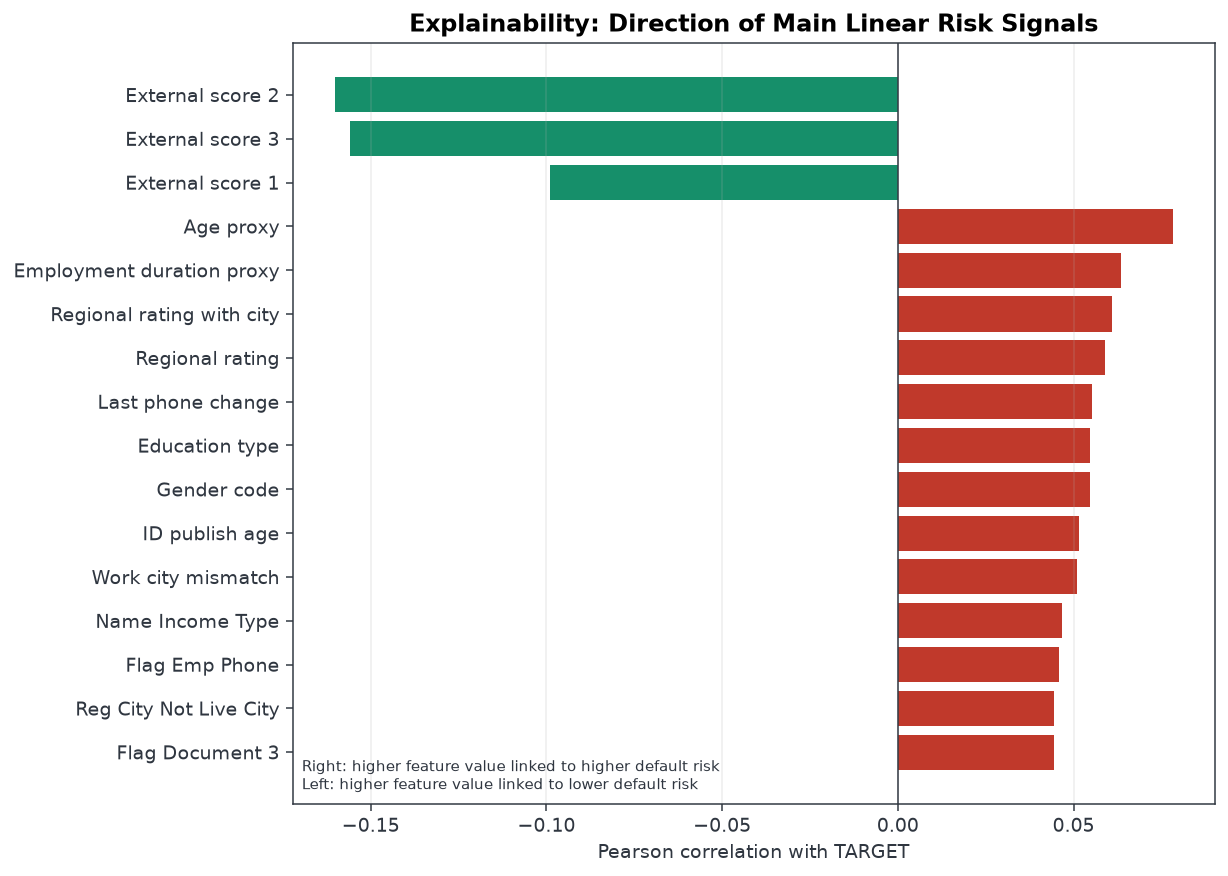
\includegraphics[width=\textwidth]{images/explainability_correlation_direction.png}
        \caption{Direção de correlação com o risco.}
        \label{fig:correlation-direction}
    \end{subfigure}
    \hfill
    \begin{subfigure}[b]{0.48\textwidth}
        \centering
        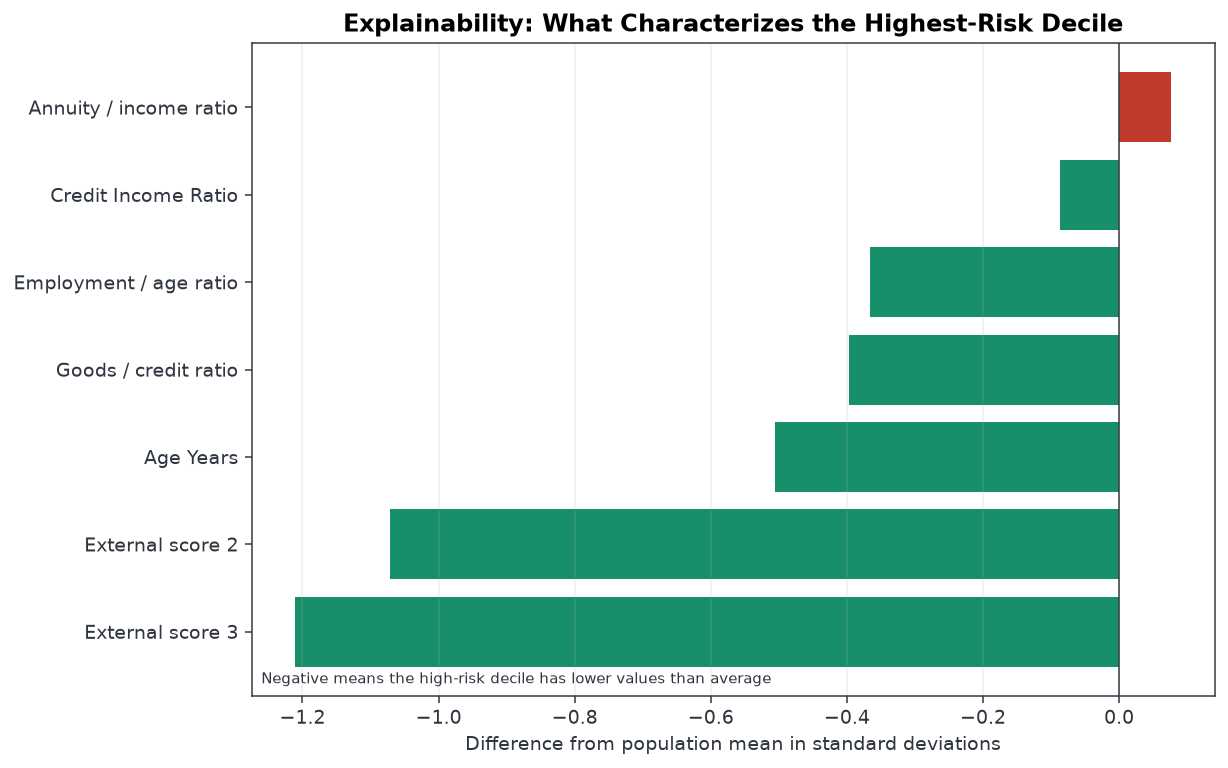
\includegraphics[width=\textwidth]{images/explainability_high_risk_profile.png}
        \caption{Perfil em desvios-padrão do decil de maior risco.}
        \label{fig:high-risk-profile}
    \end{subfigure}
    \caption{Sinais lineares e perfil multivariado associados à inadimplência.}
    \label{fig:risk-profile}
\end{figure}

\begin{figure}[H]
    \centering
    \begin{subfigure}[b]{0.48\textwidth}
        \centering
        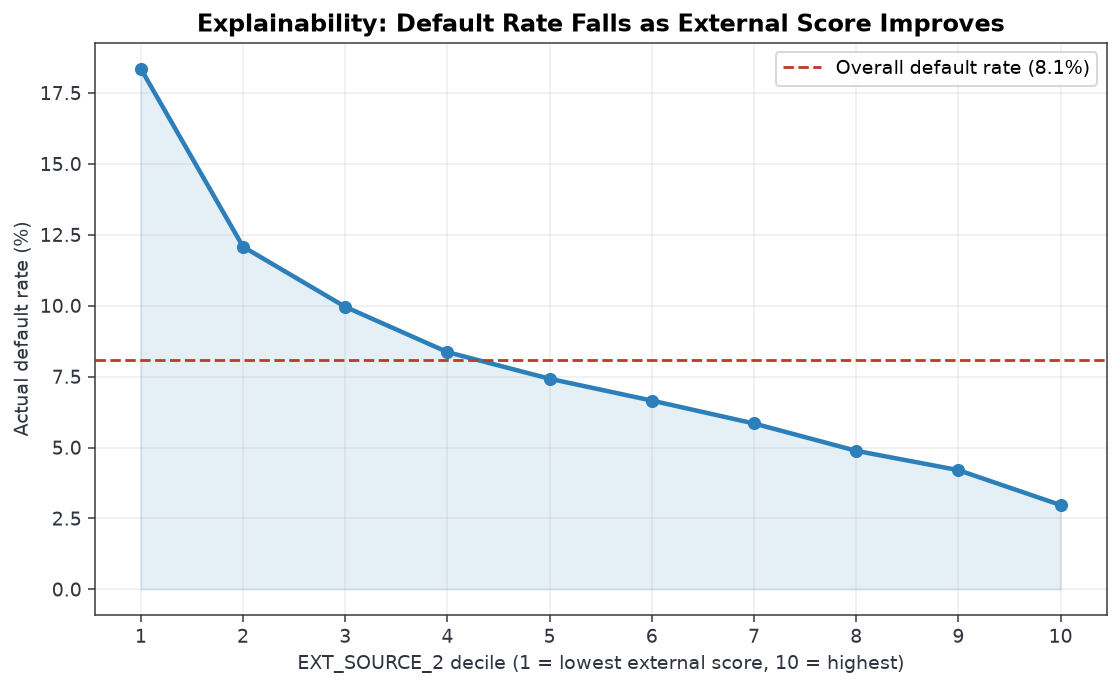
\includegraphics[width=\textwidth]{images/explainability_ext_source2_default_rate.png}
        \caption{Inadimplência por \texttt{EXT\_SOURCE\_2}.}
        \label{fig:ext-source2-decile}
    \end{subfigure}
    \hfill
    \begin{subfigure}[b]{0.48\textwidth}
        \centering
        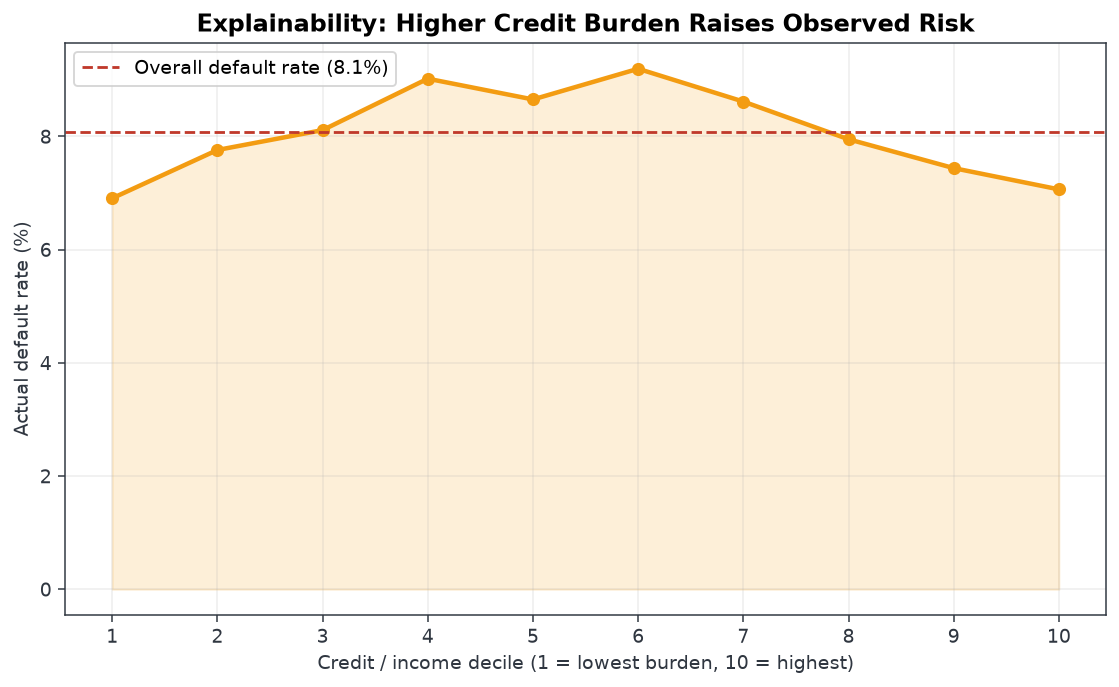
\includegraphics[width=\textwidth]{images/explainability_credit_income_default_rate.png}
        \caption{Inadimplência por razão Crédito/Renda.}
        \label{fig:credit-income-decile}
    \end{subfigure}
    \caption{Comportamento empírico da taxa real de \textit{default} isolada por decis de variáveis críticas.}
    \label{fig:risk-deciles}
\end{figure}

\subsection{Leitura dos Métodos de Explicação}
A convergência entre os métodos de explicabilidade (\textit{SHAP global}, \textit{Importância por permutação} e \textit{Importância cruzada entre modelos}) sugere uma conclusão metodológica clara: o \textit{ensemble} não dependeu de peculiaridades de implementação ou de padrões superficiais da tabela principal, mas sim de representações latentes robustas que relacionam renda, crédito, idade, emprego e histórico financeiro. 

A \textit{análise por decis de risco} traduziu essas explicações estatísticas em aplicabilidade prática, provando que o modelo é capaz de isolar o risco extremo no topo do funil. Do ponto de vista de limitações metodológicas, o projeto careceu de ferramentas de \textbf{análise local e contrafactual}. Em cenários reais de crédito, estimar como mudanças nos atributos de um cliente específico impactariam seu escore (e.g., via SHAP \textit{waterfall plots}) é o próximo passo natural para fornecer justificativas individuais auditáveis. Adicionalmente, as soluções líderes do Kaggle indicam que a criação de centenas de variáveis focadas em recência temporal e agregações condicionais produziria explicações com maior granularidade do que as obtidas neste trabalho.

\subsection{Estudo de Viés}
A presença de \texttt{CODE\_GENDER} entre os atributos mais importantes levanta uma preocupação legítima de \textbf{viés e justiça}. O modelo aprende uma associação estatística entre gênero e inadimplência, o que, embora preditivamente útil, é eticamente e por vezes legalmente problemático em concessão de crédito (muitas jurisdições proíbem o uso de gênero em decisões de crédito). Em uma aplicação de produção, seria recomendado remover atributos protegidos e auditar a diferença de desempenho entre subgrupos, aceitando a eventual perda marginal de AUC em favor da equidade.

\section{Comparação com o Ranking do Kaggle}
A validação empírica da solução ocorreu por meio da submissão oficial (\texttt{submission.csv}) na plataforma Kaggle (Figura~\ref{fig:kaggle-submission}). O sistema reportou um \textbf{Score Privado de 0,78173} e um \textbf{Score Público de 0,7828}. Essa pontuação garantiu uma posição aproximada de \textbf{3.000 entre 8.000 equipes participantes}, inserindo o modelo com folga no \textbf{top 38\%} do \textit{leaderboard}. A estabilidade entre a melhor estimativa OOF (0,7876) e o desempenho na plataforma comprova a eficácia da validação cruzada adotada contra o vazamento de dados.

\begin{figure}[H]
    \centering
    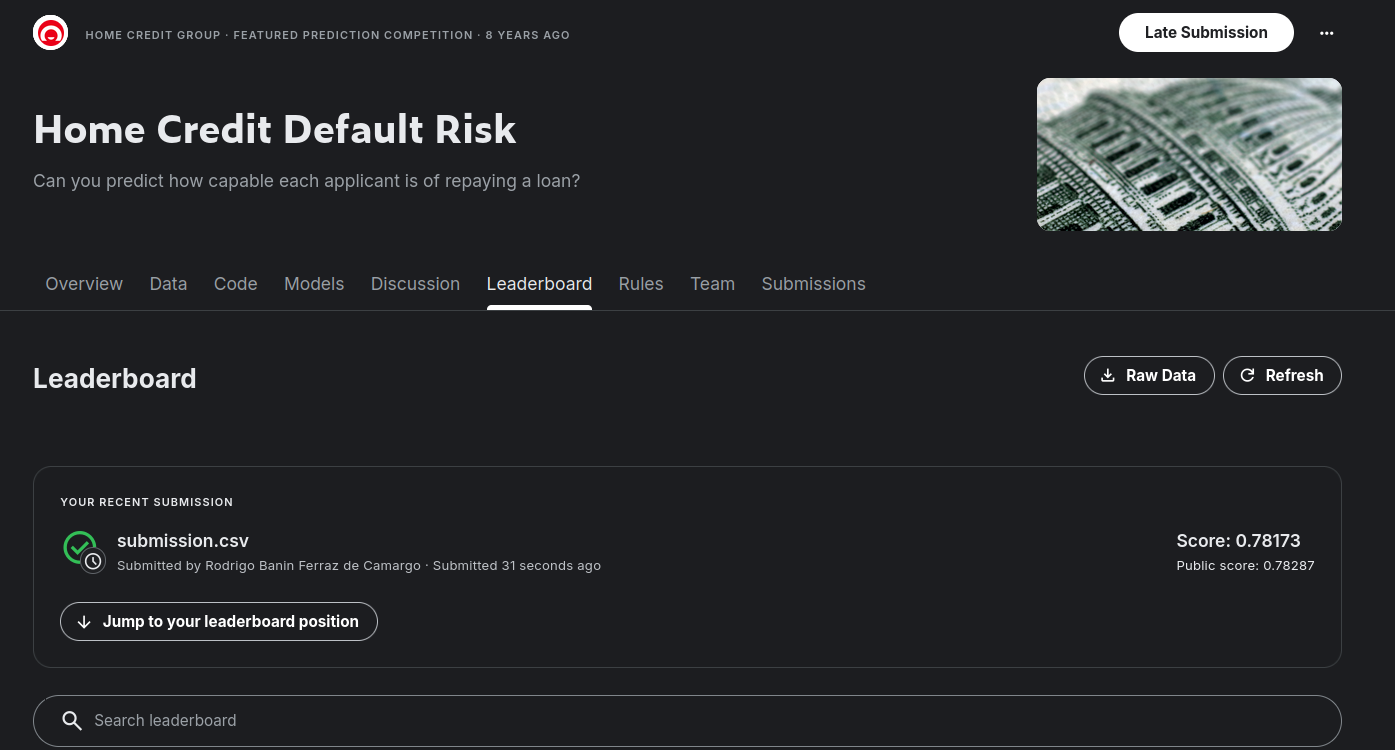
\includegraphics[width=0.67\textwidth]{images/kaggle_submission.png}
    \caption{Registro oficial da submissão no Kaggle, validando os escores público e privado alcançados.}
    \label{fig:kaggle-submission}
\end{figure}

A interpretação desse resultado deve ser desdobrada sob três perspectivas de avaliação:
\begin{itemize}
    \item \textbf{Eficácia Absoluta:} Uma AUC de $\sim$0,78 atesta que o modelo ordena com consistência o risco de clientes inadimplentes frente aos bons pagadores, entregando utilidade real para processos bancários de triagem e priorização de revisão manual.
    \item \textbf{Eficácia Relativa:} A colocação na metade superior da tabela confirma a solidez da metodologia, porém revela uma distância para a fronteira de ponta da competição. As equipes vencedoras registraram AUC privada na casa de $\sim$\textbf{0,805}, com a nota de corte do \textit{top-1\%} girando em torno de 0,800.
    \item \textbf{Diagnóstico do Gap:} A diferença de \textbf{$\sim$0,02 AUC} em relação aos líderes representa um abismo estatístico em um problema altamente saturado. Em competições maduras, saltos dessa magnitude raramente provêm de ajustes finos de hiperparâmetros ou de técnicas de \textit{ensembling} marginais.
\end{itemize}

Em suma, a distância para a liderança traduz uma assimetria na \textbf{profundidade da engenharia de atributos}. Como os modelos baseados em árvore (XGBoost, LightGBM e CatBoost) empataram tecnicamente no experimento --- sendo idênticos às arquiteturas utilizadas pelas equipes de ponta --- o gargalo metodológico não reside no algoritmo. A transição de uma solução $\sim$0,78 para $\sim$0,80 no \textit{Home Credit} exige representações mais sofisticadas da jornada financeira do indivíduo: mapeamento de janelas temporais, decaimento de risco (\textit{recência}), estabilidade de renda e mineração de subgrafos nos históricos de pagamentos e rejeições anteriores.

\section{Limitações e Oportunidades de Melhoria}
A análise crítica do projeto revela gargalos estruturais e metodológicos que definem a fronteira de expansão para trabalhos futuros:

\begin{itemize}
    \item \textbf{Engenharia de Atributos Conservadora:} Consiste no principal limitador de desempenho do modelo. A adoção de agregações estatísticas primárias (média, soma, mínimo e máximo) negligenciou dinâmicas financeiras fundamentais, como recência de atrasos, tendências temporais, contagens condicionais de status e janelas móveis --- fatores algorítmicos que classicamente distinguem as soluções de topo neste domínio.
    \item \textbf{Otimização e \textit{Stacking}:} A média ponderada (\textit{blend}), embora resiliente, subutiliza a complementaridade residual dos classificadores. A implementação de um meta-modelo treinado sobre as predições OOF (\textit{Stacking}), aliada à exploração bayesiana sistemática de hiperparâmetros (via \texttt{Optuna}), extrairia o teto de performance de cada \textit{booster} base.
    \item \textbf{Representação em \textit{Deep Learning}:} A performance deprimida da rede MLP evidencia a limitação de topologias genéricas em domínios tabulares esparsos. O uso de arquiteturas dedicadas (como \textit{TabNet} ou \textit{FT-Transformer}) e o mapeamento de variáveis categóricas via \textit{embeddings} densos tornaria a rede um componente mais competitivo no \textit{ensemble}.
    \item \textbf{Explicabilidade Local e Calibração:} O estudo focou na interpretação global (\textit{feature importance}). A transposição para o negócio exigiria explicabilidade em nível de instância (\textit{e.g.}, SHAP \textit{waterfall}, análise contrafactual) para gerar justificativas auditáveis cliente a cliente, além de métodos de calibração probabilística absoluta (Isotônica/Platt) para corrigir as distorções inseridas pelo rebalanceamento de classes.
    \item \textbf{Governança e Mitigação de Viés:} A relevância estatística do atributo protegido \texttt{CODE\_GENDER} sinaliza desafios éticos e regulatórios prementes. Em um cenário de produção real, seria imperativa a remoção de características protegidas e a condução de uma auditoria de paridade algorítmica rigorosa (avaliando disparidades em AUC, taxas de falsos positivos e falsos negativos entre subgrupos).
\end{itemize}

\section{Conclusão}
Este trabalho consolidou uma abordagem estruturada e uma análise crítica profunda para o desafio \textit{Home Credit Default Risk}, a partir de um ecossistema relacional de sete tabelas, foi desenvolvida uma pipeline de engenharia de características que expandiu a dimensionalidade preditiva de $\sim$120 para $\sim$350 variáveis. A avaliação rigorosa de seis modelos-base sob validação cruzada estratificada revelou o XGBoost como o estimador isolado mais forte (\textbf{AUC OOF de 0,7876}), enquanto o \textit{ensemble} alcançou a melhor métrica de \textit{Average Precision} (\textbf{0,2832}), fundamental em cenários desbalanceados. A submissão oficial (\texttt{submission.csv}) registrou \textbf{Score Privado de 0,78173} e \textbf{Score Público de 0,7828}, garantindo presença no \textbf{top 38\%} global ($\sim$3.000/8.000 participantes).

Para além do desempenho no \textit{leaderboard}, o estudo extraiu uma interpretação de negócios empiricamente validada: o risco de inadimplência neste domínio é governado substancialmente por escores externos pré-existentes e suas interações, fortemente modulados por relações demográficas (idade/emprego), histórico de pagamentos e razões de crédito. Essa narrativa foi corroborada pela convergência analítica entre a decomposição SHAP global, importância por permutação e análise operacional por decis. Contudo, o limite atual da solução reside na explicabilidade: possuímos um mapa global claro das decisões, mas careceu-se de ferramentas de inferência local e contrafactual para fundamentar recusas de crédito cliente a cliente.

A distância de aproximadamente \textbf{0,02 ponto de AUC} para as soluções que lideram a competição ($\sim$0,80 AUC) reforça o principal aprendizado do projeto: o hiato não é de natureza algorítmica, uma vez que operamos com as mesmas famílias de \textit{gradient boosting} (XGBoost, LightGBM, CatBoost) adotadas pela elite do Kaggle, mas sim representacional. O aprimoramento dessa solução e a redução do risco sistêmico exigem transcender agregações conservadoras, migrando para uma engenharia de atributos focada em recência temporal, decaimento de risco de atrasos e agregações transacionais condicionais. Conclui-se que, em modelagem de crédito, elevar o patamar de predição é uma tarefa inerentemente dependente da construção de descrições mais ricas e precisas do comportamento financeiro longitudinal do cliente.

\end{document}
